%!TEX root=../GaugeCNNTheory.tex


\section{\lr{CNN}های هموردای دورانی در فضاهای اقلیدسی سوراخ‌دار}
\label{sec:instantiations_euclidean_polar}

\begin{figure}
	\centering
	\begin{subfigure}[b]{0.47\textwidth}
		\centering
		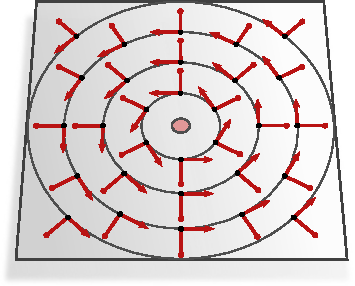
\includegraphics[width=.7\textwidth]{figures/G_structure_R2_no_origin_SO2.pdf}
		\captionsetup{format=hang, width=.82\textwidth}
		\caption{\small
			$\{e\}$-ساختار ناوردای $\SO2$ که به طور ضمنی توسط \citet{finzi2020generalizing} فرض شده است.
		}
		\label{fig:G_structure_R2_no_origin_SO2}
	\end{subfigure}
	\hfill
	\begin{subfigure}[b]{0.47\textwidth}
		\centering
		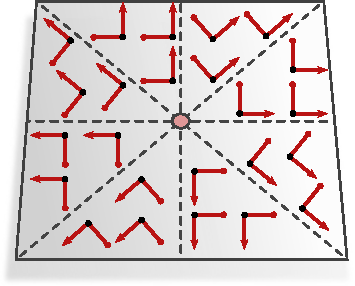
\includegraphics[width=.7\textwidth]{figures/G_structure_R2_no_origin_C8.pdf}
		\captionsetup{format=hang, width=.78\textwidth}
		\caption{\small
			$\{e\}$-ساختار ناوردای $\operatorname{C}_8$ که به طور ضمنی توسط \citet{chidester2019rotation} فرض شده است.
		}
		\label{fig:G_structure_R2_no_origin_C8}
	\end{subfigure}
	\caption{\small
		دو مثال از $\{e\}$-ساختارها در صفحه سوراخ‌دار $\Euc_2 \backslash \{0\}$ که
		۱) تحت دوران حول مبدأ $\{0\}$ ناوردا هستند و
		۲) متشکل از چارچوب‌های راست‌هنجار نسبت به متریک اقلیدسی استاندارد هستند.
		کانولوشن‌های $\GM$ متناظر، هموردای دورانی هستند اما هموردای انتقالی نیستند (در واقع، $\Euc_2 \backslash \{0\}$ حتی انتقال‌ها را نمی‌پذیرد).
	}
	\label{fig:G_structures_R2_no_origin}
\end{figure}


مدل‌های موجود در ردیف‌های (۲۷-۳۰) جدول~\ref{tab:network_instantiations}
یک جایگزین جالب برای کانولوشن‌های هموردای دورانی در فضاهای اقلیدسی سوراخ‌دار $\Euc_d\backslash\{0\}$ ارائه می‌دهند.
آنها بر \emph{$G$-ساختارهایی تکیه دارند که تحت دوران حول مبدأ انتخاب شده $\{0\}$ ناوردا هستند}، همانطور که به عنوان مثال در شکل~\ref{fig:G_structures_R2_no_origin} به تصویر کشیده شده است.
با مشخص کردن یک مبدأ مرجح، این مدل‌ها ویژگی هموردایی انتقالی را از دست می‌دهند.%
\footnote{
	این مشکل را می‌توان با ترکیب شبکه با یک شبکه پیش‌بینی‌کننده مبدأ ناوردای انتقالی حل کرد~\cite{esteves2017polar}.
	توجه داشته باشید که هموردایی دورانی مدل ترکیبی تنها در صورتی حفظ می‌شود که این پیش‌بینی‌کننده مبدأ، $\SE{d}$-هموردا باشد.
}
با این حال، اگر $G$-ساختار علاوه بر این تحت مقیاس‌بندی نیز ناوردا باشد، که به عنوان مثال زمانی که توسط مختصات فراکروی با یک مؤلفه شعاعی لگاریتمی القا می‌شود، صادق است (همانطور که در شکل~\ref{fig:G_structure_R2_no_origin_logpolar} نشان داده شده)، مدل‌ها نسبت به حاصلضرب مستقیم $\SO{d} \!\times\! \Scale$ از گروه دوران و مقیاس‌بندی هموردا می‌شوند.
به طور مشابه، $G$-ساختارهای ناوردای دورانی و بازتابی، که در شکل~\ref{fig:G_structure_R2_no_origin_O2} به تصویر کشیده شده‌اند، بر هموردایی $\OO{d}$ کانولوشن‌های $\GM$ متناظر دلالت دارند.


این مدل‌ها به دو صورت به \lr{CNN}های کروی، که در بخش~\ref{sec:instantiations_spherical} در ادامه مورد بحث قرار می‌گیرند، مرتبط هستند.
اولاً، آنها $G$-ساختارهای ناوردای دورانی را روی $\Euc_d \backslash \{0\} \,\cong\, S^{d-1} \!\times \R^+$ فرض می‌کنند، که می‌توان آنها را متشکل از چندین $G$-ساختار ناوردای دورانی روی پوسته‌های کروی ${(d -\! 1)}$-بعدی $S^{d-1}$ در شعاع‌های مختلف در نظر گرفت.
بنابراین می‌توان این مدل‌ها را به عنوان \lr{CNN}های (فرا)کروی با یک بعد شعاعی اضافی~$\R^+$ در نظر گرفت~\cite{ramasinghe2019representation}، که در شکل~\ref{fig:G_structure_R3_no_origin} برای حالت $d=3$ بعد به تصویر کشیده شده است.
ثانیاً، سیستم‌های مختصات قطبیِ \cite{esteves2017polar,finzi2020generalizing,chidester2019rotation} (شکل‌های~\ref{fig:G_structures_R2_no_origin} و~\ref{fig:G_structure_R2_no_origin_logpolar}) $G$-ساختارهایی را القا می‌کنند که همان نوع تکینگی را در مبدأ خود نشان می‌دهند که \lr{CNN}های کروی سوراخ‌دار در شکل~\ref{fig:G_structure_S2_2} در قطب‌ها دارند.
توجه داشته باشید که صفحه اقلیدسی سوراخ‌دار $\Euc_2 \backslash \{0\}$ و کره سوراخ‌دار $S^2 \backslash \{n,s\}$ (با قطب‌های شمال و جنوب $\{n,s\}$ حذف شده) هر دو از نظر توپولوژیکی معادل یک استوانه $S^1 \times \R^+ \cong S^1 \times \R$ هستند و $\{e\}$-ساختارهای استوانه‌ای که در شکل‌های~\ref{fig:G_structure_R2_no_origin_SO2}، \ref{fig:G_structure_R2_no_origin_logpolar} (چپ) و~\ref{fig:G_structure_S2_2} به تصویر کشیده شده‌اند، دیفئومورفیک هستند.


یک تفاوت عمده در مقایسه با شبکه‌های $\SE{d}$-هموردا از بخش قبل این است که مدل‌های بخش فعلی فقط \emph{به‌صورت سراسری} حول مبدأ $\SO{d}$-هموردا هستند به جای اینکه \emph{به‌صورت محلی} $\SO{d}$-هموردا ($\SO{d}$-راهبری‌پذیر) باشند.
در حالی که مدل‌های هموردای سراسری به کرنل‌های $\SO{d}$-راهبری‌پذیر نیاز ندارند، آنها همچنان حداقل به کرنل‌های $\SO{d-1}$-راهبری‌پذیر نیاز دارند.
این به این دلیل است که $\SO{d}$ یک کلاف $\SO{d-1}$ روی پوسته‌های کروی $S^{d-1} \cong \SO{d}/\SO{d-1}$ است که $G$-ساختار روی آن باید نسبت به دوران $\SO{d}$ هموردا باشد.
برای $d=2$ این امر به $\{e\}$-ساختارها و کرنل‌های غیرراهبری‌پذیر اجازه می‌دهد زیرا $\SO{d-1} = \SO{1} = \{e\}$؛ به شکل~\ref{fig:G_structures_R2_no_origin} یا~\ref{fig:G_structure_R2_no_origin_logpolar} مراجعه کنید.
برای $d=3$ این امر حداقل به یک $\SO{d-1} = \SO{2}$-ساختار روی پوسته‌های کروی جداگانه نیاز دارد، که در شکل~\ref{fig:G_structure_S2_1} به تصویر کشیده شده است.


پس از این ملاحظات کلی، در ادامه به طور خلاصه مدل‌های جداگانه روی $\Euc_d \backslash \{0\}$ را که در مقالات یافت می‌شوند، از دیدگاه \lr{CNN}های مستقل از مختصات مرور خواهیم کرد.
ما با مدل‌های ردیف (۲۷) جدول~\ref{tab:network_instantiations} شروع می‌کنیم، که نسبت به دوران‌های $\SO2$ حول یک مبدأ انتخاب شده از~$\Euc_2$ هموردا هستند و با مدل‌های ردیف (۲۸) ادامه می‌دهیم، که علاوه بر آن هموردای مقیاس هستند.
شبکه فهرست شده در ردیف (۲۹)، که در آخر آن را مورد بحث قرار می‌دهیم، به صورت سراسری حول مبدأ~$\Euc_3$ هموردای $\OO3$ است.